\documentclass[12pt,oneside,openright]{report}

\usepackage[utf8]{inputenc}
\usepackage[scaled]{helvet}
\usepackage{subcaption} % Add the subcaption package for subfigures
\usepackage{dirtytalk} %quoting package
\renewcommand\familydefault{\sfdefault} 
\usepackage[T1]{fontenc}
\usepackage{fancyhdr,xcolor}

\usepackage{graphicx} % Add the graphicx package for including images
\usepackage{geometry}
\usepackage{amsmath} % Add this line to your LaTeX preamble to use \text
\usepackage{changepage}
\usepackage{pdfpages}
\usepackage{afterpage}
\usepackage{caption}
\usepackage{float}
\usepackage{xcolor}

\usepackage[style=authoryear,backend=biber]{biblatex}
\addbibresource{bibliog.bib}
\usepackage[colorlinks=true,linkcolor=black,anchorcolor=black,citecolor=black,filecolor=black,menucolor=black,runcolor=black,urlcolor=black]{hyperref}\usepackage{graphicx}
\usepackage{adjustbox}
\geometry{
  a4paper,
  left=20mm,
  right=20mm,
  top=3cm,
  headheight=4cm,
  bottom=3.5cm,
  footskip=3cm
}

\renewcommand*{\bibfont}{\footnotesize}

\newcommand{\changefont}{
    \fontsize{18}{16}\selectfont
}
\definecolor{boxcl}{HTML}{1188BB}
\definecolor{tubred}{HTML}{1188BB}



\begin{document}

\begin{titlepage}
    \centering
    % Include the image with a width of one-third of the page
    
\includegraphics[width=0.5\textwidth]{Hu-logo.png}
    \vspace{2cm}
    
    {\huge \textbf{Multisensory Integration in Virtual Reality: Effects of Passive Haptic Stimulation}\par}
    \vspace{2cm}
    {\LARGE Master Thesis\par}
    \vspace{0.5cm}
    {\textbf{submitted in fulfilment of the requirements for the degree}\par}
    Master of Science (M.Sc.)\par
    {\textbf{in the master's program ``Mind and Brain''}\par}
    \vspace{1.5cm}
    {\textbf{Humboldt-Universität zu Berlin}\par}
    {\textbf{Berlin School of Mind and Brain}\par}
    \vfill
    \raggedright
    \begin{tabular}{ll}
        \textbf{Handed in by}: & Benjamin Dupré \\
        \textbf{Date of birth:} & 26.04.1986\\
       \textbf{ Address:} & Hoppestraße 16, 13409, Berlin \\
    \end{tabular}
    \vfill
    \begin{tabular}{ll}
        \textbf{1. Supervisor:}& Dr. Michael Gaebler \\
        \textbf{2. Supervisor:}& Professor Dr. Arno Villringer  \\
    \end{tabular}
    \vfill
    {Berlin, \today \par}
\end{titlepage}

\newpage
%\thispagestyle{empty}
\section*{\centering Acknowledgments}

\begin{adjustwidth}{1cm}{1cm}
%\begin{center}

    I would like to express my sincere gratitude to Dr Michael Geabler and Prof. Dr Arno Villringer for their advice and support in making this thesis possible. Many thanks to Max Hellrigel-Holderbaum for his friendly editing and references, as well as to Zaynep Akbal and Tim Julian Möller for generously sharing their expertise and time.

    I am deeply grateful for the support provided by the Max-Plank Institute, specifically from Zeynep Akbal and Arno Villringer (NRO-228), and Study-DB (0218807).
    
%\end{center}
\end{adjustwidth}

\clearpage

\section*{1. Introduction}
%\subsection*{1.1 Problem \& Significance}

Interoception intricately weaves together the everyday physiological and cognitive mechanisms responsible for perceiving, comprehending, and integrating internal bodily cues. This continuous mapping of our dynamic internal state, operating across both conscious and unconscious levels, distinguishes interoception, exteroception (perception of the environment) and proprioception (awareness of body position) from each other. In doing so Interoceptive signals, additionally, also influence our interaction with the environment, thereby impacting our perception of the world. This thesis delves into this particular aspect. These signals not only relay information about bodily conditions but also significantly influence our perception and interaction with the environment, therefore shaping our reality \parencite{Galvez-Pol2022-vb}.

Immersive Virtual Reality (IVR) is a computer-generated environment that can be interacted in a seemingly real or physical way as provided by the electronic equipment. IVR replaces our visual, proprioceptive, auditory and touch signals, replacing the physical with computer-mediated input. Thus, IVR wraps individuals in a computer-created environment, potentially creating a sense of presence. This notion of presence signifies the degree to which individuals realistically respond to these virtual environments, spanning from emotional and behavioural reactions to groundlike psychophysical responses \parencite{SanchezVives2005FromPT}.

In the realm of psychophysics, studies traditionally explore the correlation between the physical world and its sensory representations. These experiments often involve very simple experimental setups that allow for precise measurement of a single stimulus (intensity, length, etc.). Also, they involve a limited number of highly trained subjects contributing extensive observations \parencite{KINGDOM2012234,WASKOM2019100}. Conversely, investigations into higher-level emotional and behavioural aspects typically recruit larger, less specialized cohorts, focusing on population-level analyses \parencite{WASKOM2019100}.

Despite the 40-year evolution of IVR, the majority of research has emulated physical reality, assessing skill transference and similar aspects. However, IVR holds great potential for multisensory research and looks into interoceptive, exteroceptive, and proprioceptive signal integration. Yet, it has been primarily viewed as a medium for simulating existing experiences rather than exploring its relative non-realism. The opportunity in VR holds also in the fact that we can with high precision manipulate sensory information while leaving proprioceptive and interoceptive signals unchanged. We can, therefore,  build experimental setups to understand how all signals used by our brain and bodies integrate to form what we call reality \parencite{Vasser2020GuidelinesFI, deGelder2018VirtualRA}.

This thesis proposes an experimental VR setup using a multisensory integration study as a reference and platform for exploring this largely uncharted territory. To be able to use IVR and its "lack of realism" we need to have very previous psychophysical experiment results. The subsequent sections delve into the specific findings categorized into psychophysical and cognitive studies, which build up an intended contrast to the reference study that forms the central part of this thesis. Later this stresses the relevance of using IVR as an important new tool Conitive Psychophics. Central advantages of IVR for Cognitive Psychophysics especially include a much better ecological validity and broader generalizability beyond narrow experimental settings \parencite{NASTASE2020117254}.

\subsubsection*{Perception \& Psychophysics}

Psychophysical research concerns itself with the relationship between physical phenomena and their perceptual effects. Experiments in Psychophysics typically focus on a single perceptual modality, employing high-precision measurements. Within the Interoception literature, a subset of psychophysical studies centres on the cardiac cycle, specifically the events during each heartbeat (systole and diastole). These studies present perceptual stimuli synchronized with a specific cardiac phase (phase-lock) and assess changes in reaction time (RT) or detection task performance.

This body of research indicates that interoceptive signals significantly influence our perception of external signals in touch, vision, and auditory cues. In the somatosensory domain, detecting near-threshold stimuli with higher accuracy occurs during the diastolic phase compared to systole \parencite{esra_p, AL2021118247, Grund643, motyka}. For vision and auditory stimuli, diastole improves accuracy and reaction time compared to systole \parencite{SALTAFOSSI2023108642}. However, real-life stimuli rarely occur in a single modality. Thus, the question remains, whether and how interoceptive signals impact multisensory integration.

My reference study aims to answer this question by replicating some results from psychophysical experiments, contributing to the validation of using immersive virtual reality (IVR) and passive haptic stimuli. \textcite{SALTAFOSSI2023108642} investigates the integration of multiple simultaneous sensorial modalities (interoceptive and exteroceptive). Forty healthy participants performed a detection task involving unimodal (Auditory, Visual, Tactile) and bimodal (Audio-Tactile, Audio-Visual, Visuo-Tactile) stimuli. These stimuli were presented either 250 ms after the R-peak of the electrocardiogram (systole) or 500 ms after (diastole). The study found a general impact of cardiac cycle phases on detecting both single and combined stimuli, with reaction times being faster during diastole.

Importantly, I employ and replicate the well-known Race Model Inequality (RMI) and response times (RT), to measure multisensory integration. Redundant signal effects refer to the fact individuals respond faster to redundant sensory signals than unisensory signals. One proposed explanation is the Race Model Inequality (RMI), suggesting that evidence for each signal accumulates separately in parallel decision units (e.g., one for audition and one for vision), and the first unit to reach its threshold triggers a behavioural response like in the experiment just mentioned. A violation of this expected preposition would indicate sensory modality integration. 

As measured in my reference study, the diastolic cardiac phase enhances the integration of sensory signals (e.g. measured as reaction times being faster for stimuli presented during diastole, compared
to systole). Audio-Tactile and Visuo-Tactile stimuli show higher integration during diastole compared to systole, unlike Audio-Visual stimuli (e.g. measured as the CDF for an RT $t$). This observation suggests a potential specificity in the influence of the cardiac phase on multisensory integration, particularly in stimuli involving somatosensory inputs (e.g., tactile).

All studies so far involve the passive presentation of stimuli and phase-locked conditions. Nevertheless, in our daily lives, stimuli come to us in a constant stream through multiple modalities. Thus, two important questions remain to be answered: Would a more naturalistic stimuli interaction still reveal a modulation role of interoceptive signals? Can VR help us answer this further? By the end of the thesis, we will understand what conditions need a VR experimental set-up to answer these two questions. 

\subsubsection*{Interocpetion \& Cognition}

The second group of studies delves into higher cognitive functions. A study by \textcite{Garfinkel2013-cy} aims to measure if there's a difference in how we memorize a word presented during a specific cardiac phase. Words were shown within a limited attentional timeframe synchronized with different cardiac phases. This aspect of the experiment sought to investigate whether natural baroreceptor activity affects word detection and subsequent memory. The study revealed that recalling words presented during systole is lower compared to words presented at diastole. This memory decrease during systole is more pronounced for words identified with low confidence and heightened among individuals with lower interoceptive sensitivity, measured through a heartbeat counting task.

Another two studies aim to understand if the way in which we actively sample the world is similarly modulated by interoceptive signals. The first study focuses on exploring the role of the heartbeat in active information sampling, investigating whether humans unconsciously arrange their environment to encounter pertinent signals during preferred cardiac phases. In the visual memory experiment's encoding phase, participants navigated through a series of emotional pictures, aiming to memorize them for a subsequent recognition test. Through self-paced key presses, they initiated the display of brief (100 ms) images. The study's findings unveil fluctuations in self-triggered picture onsets throughout the cardiac cycle, notably heightened during cardiac systole, yet without impacting memory performance. This leads the study to conclude that active information gathering incorporates signals related to the heartbeat \parencite{Kunzendorf2019-vz}. A similar study confirms these findings. It was achieved by presenting participants with arrays to compare in size. They measured participants' eye movements, heart rate, and response times. The authors similarly found a significant coupling of saccades, subsequent fixations, and blinks with the cardiac cycle. They observed that more eye movement occurs during systolic phases while more fixation happens during diastolic phases, thus demonstrating an active perceptual role \parencite{GalvezPol2018ActiveSI}.

So far we have discussed interoceptive signal's effects on exteroceptive perception. We have also seen these signals enhance multisensory integration, particularly in stimuli involving somatosensory (e.g., tactile) inputs. Additionally, when observing these interoceptive signals, we have noted an increase in cognitive behavioural outcomes, such as word recognition and promotion of active information sampling behaviour. But how do all of these separate facts integrate together? Are there more general patterns to be found in multisensory integration that may be assessed in experiments using IVR? I focus on that question below. 

\subsubsection*{Inmersive Virtual Reality as the new tool for psychophysical investigations of cognition}

Several previous papers propose a theoretical account that includes, to some extent, the before-discussed findings. These theoretical accounts propose an interoceptive predictive framework. The framework suggests that repetitive bodily signals, such as the respiration cycle, could be predicted and suppressed to avert conscious perception. If this framework is true, it would suggest that external stimuli are inadvertently suppressed. This suppression is relevant because it offers an "explanation" that includes all previous findings and a general explanation for how the body and mind work (as it is a subexplanation nested within the broader predictive coding processing theory) \parencite{AL2021118247, SALTAFOSSI2023108642, Allen2022}.

Another paper presents a comprehensive computational interoceptive predictive framework \parencite{Allen2022}. A particular strength of this paper is that it uses a more refined formalization than the one before, employing Markov Decision Processes. The agents deduce their pursued policy (relaxation or arousal) to create the most effective mapping (from state to sensation in the risk minimization problem). Operationally defining policies involves transitioning between interoceptive states. For instance, in a relaxed state, the probability shifts among cardiac states, resulting in two phases of diastole and one of systole. In contrast, arousal triggers an immediate shift from the initial diastolic state to systole. Essentially, arousal prompts cardiac acceleration and prolongs the time spent in systole on average. One assumption of the article is that precise visual information is available only during specific phases of the cardiac cycle, contingent upon one's arousal state. Among its findings, the paper demonstrates the model's ability to replicate various psychological and physiological phenomena found in the interoceptive inference literature and provides a means to test such a model.

These are some examples that offer a theoretical account of the fact that interoceptive signals modulate external signal processing. These descriptions can be applied more easily to perceptual phenomena than cognitive phenomena. During the study of cognitive processes, experimental remoteness is more of an issue (In general, a problem composed of two elements: cognitive processes are less accessible to manipulation than physical processes and the amount of uncertainty for the measurement and experimental manipulation of cognitive processes increases). Cognition is at the end of a long change of interactions that starts with sensory input and can be observed through behaviour or self-report. In this way, the distance between the external variables manipulated and the behaviour observed is greater and without careful consideration, the uncertainty of an experimental manipulation can lead towards a complete miss of the cognitive process of interest \parencite{WASKOM2019100}.

To diminish the problem of experimental distance in psychology an alternative is cognitive psychophysics. Three key points should be adhered to. Firstly, to emphasize tasks where expert observers make threshold-level judgments about experimental stimuli, enabling precise control. Secondly, adopt a conceptual orientation focused on quantification as a primary goal of experimental design. Finally, place formal computational models centrally in the analysis and interpretation of behavioural and body-brain data \parencite{WASKOM2019100}. A VR system offers a way to address all of these issues simultaneously. In this thesis, we exploit some of these advantages. 

The benefits of using VR are not only limited to its use in cognitive psychophysics. During a virtual reality (VR) experience, an interaction occurs between sensory systems and higher cognition. Leveraging the limitations of the VR world, rather than its richness, provides a unique opportunity to explore the design and mechanisms of brain systems underlying phenomena such as multisensory integration and their intricate characteristics. For instance, a somatosensory signal designed for VR can systematically differ from a real-life somatosensory stimulus. Rather than striving for heightened realism, researchers can create various 'impoverished' versions of real somatosensory signals by systematically manipulating their attributes and measuring their intensity. Investigating these manipulations is akin to developing and testing a set of hypotheses to unravel the properties of the underlying functional design of multisensory integration and its interoceptive and exteroceptive foundations \parencite{deGelder2018VirtualRA}.

In this thesis, the initial phase of this approach involves replicating previous studies and aligning the experimental conditions more closely with real-world situations.


\subsubsection*{The Thesis}

We propose a novel experimental setup utilizing Immersive Virtual Reality (IVR). Studies involving IVR and electrophysiological devices are relatively recent, primarily due to technical limitations hindering signal acquisition \parencite{Klotzsche2023,Kisker2024InducedOB}. Nonetheless, this type of study can help narrow the experimental gap by accurately measuring input and behavioural responses, even if the stimulation is not precisely correct.

Traditional experiments have relied on visual displays and head-controller movement tracking, attempting to mimic reality as closely as possible (e.g. by translating classical research paradigms to virtual reality (VR) or advancing them within these immersive settings \parencite{Kisker2024InducedOB}). Our study introduces a VR head-mounted display with Electrocardiogram (ECG) monitoring and haptic gloves. Integrating these devices presents challenges, both technical and in terms of alignment with existing literature.

The primary objective is to validate the haptic feedback provided by the gloves in the context of multisensory integration. A secondary goal is to replicate the RMI findings from \textcite{SALTAFOSSI2023108642}(I'll call the study by Saltafossi et al. 2023 the reference study.). This study showed an increase in multisensory integration for touch-visual and touch-audio cues in the context of interoceptive stimuli. The RMI serves to dismiss the idea that quicker response times (RTs) could be explained by separate processing (i.e., Race Model). It posits that the combined RT distribution for redundant stimuli never surpasses the total RT distribution for the individual unimodal stimuli. Rejecting this notion indicates interactions across multiple senses.

The former enhances our understanding of using IVR as a tool for psychophysical investigations of cognition, while the latter nests our research within previous findings. To the best of my knowledge, the reference study is the only one using RMI analysis to explore multisensory integration, considering interoceptive and exteroceptive signals.

Considerable distinctions exist between the stimuli employed in this study and the referenced study. In this investigation, vision is the sole unimodal signal, while the reference study includes measurements for single modalities in vision, touch, and audio. Additionally, in the reference study, touch is provided as a small electrical charge determined for each participant using the method of limits. In our study, touch is simulated by a vibrotactile glove. For the scope of this thesis inquiry primarily focuses on conditions related to the tactile sense.

By investigating the influence of passive haptic stimuli on response time within a motor-memory task, this study replicates the principal observations outlined in heart cycle multisensory integration literature \parencite{SALTAFOSSI2023108642}, confirming IVR as a means of developing psychophysical investigations of cognition.

\section*{2. Methods}
\subsection*{Participants}
The call for participants targeted healthy, non-smoking German-speaking individuals between 18 and 30 years old. They were contacted and recruited via e-mail, using the database of Max-Plank CBS for registered participants. Participants were required to be righthanded and without neurological or psychiatric illnesses (e.g. epilepsy). When taking part in the experiment participants were paid 9 € the hour. The experimental session took 2.5 hours on average. The participant came to the laboratory in October 2020  the study was conducted following the declaration of Helsinki. All participants provided informed written consent. 

Initially, 23 individuals answered and participated in the study, but ultimately, only 20 participants were included in the final sample. Among the three excluded individuals, two failed to complete all necessary questionnaires, while the third exceeded the age limit of 30. Notably, a greater number of women (15) responded to the call compared to men (5). The average age across the sample hovered around 25 years, with a slight deviation observed in one participant ($\mu=25.1, \sigma=6.3$).

\begin{figure}[h]
    \centering
    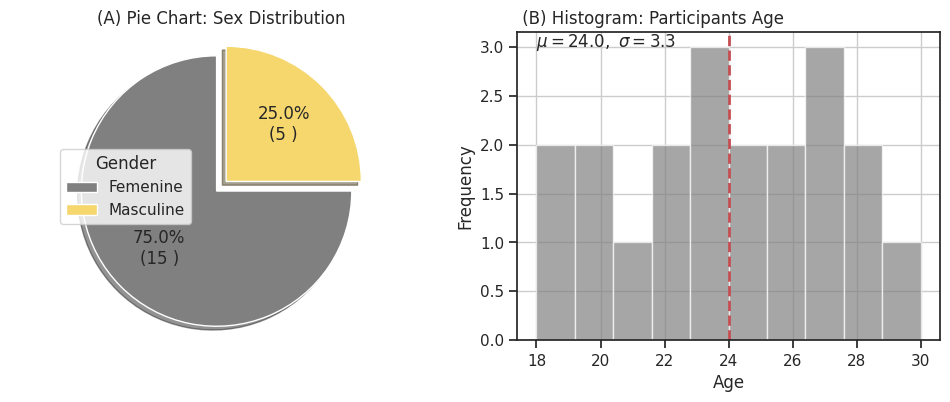
\includegraphics[width=15cm]{/home/perdices/Dokumente/Github/m-b_thesis/HU Thesis/figures/participants.png}
    \captionsetup{justification=justified, margin={2cm,2cm}, font={small}}
    \caption{Participant's Distribution}
    \label{fig:mesh1}
\end{figure}

    
\subsection*{Materials}

\subsubsection*{Electrocardiogram (ECG):}
Heart rate data was collected using an Arduino Uno and a SparkFun Single Lead Heart Rate Monitor - AD8232. The data was transferred through a USB 2.0 connection and integrated into the Unity log file at a frequency of 133 Hz. Compared to a clinical ECG, this device entails a serial interface that can send triggers via USB directly to a computer and software (e.g. Unity, Matlab) with minimal delay due to its architecture. Its software and hardware are open-source and publicly available \parencite{TimsECG}.

\subsubsection*{Head Mounted Display \& Lighthouses:}
The VR setup included a HTC Vive head-mounted display (HMD) with two lighthouses. The headset specifications included a Dual AMOLED 3.6" diagonal display, with 1080 x 1200 pixels per eye (2160 x 1200 pixels combined), a 90 Hz refresh rate, and a 110-degree field of view. The lighthouses are equipped with SteamVR Tracking, G-sensors, gyroscopes, and proximity sensors. Both the HMD and lighthouses are connected using USB 2.0. For this study, the VR controllers were not used, and instead, hand tracking was performed using the Leap Motion sensor.

\subsubsection*{Leap Motion Controller:}
This device was used to track the position of the hands. The Leap Motion Controller has a field of view of 150x120 degrees, with a variable range of roughly 80 cm (arm's length). It weighs 32 grams and is mounted on the HMD. The device features two 640x240 infrared cameras with a frame rate of 120 fps.

\subsubsection*{Data Gloves:}
The data gloves used in the study are equipped with magnetic sensors and connected to Unity using a micro USB connection. These gloves provide haptic feedback through 10 vibrotactile actuators, offering a wide range of tactile sensations with 1,024 levels of intensity. The gloves also incorporate complete finger tracking using six 9-axis Inertial Measurement Units (IMUs). These IMUs enable precise tracking of finger movements, allowing for accurate gesture recognition and enhanced interaction in virtual environments. The datagloves and finger tracking were interfaced from the experimental code using the UnityDll.Motion and c\# NeuroDigital licensed code (NeuroDigital Technologies, 2018).


\subsection*{Task}

In the following, I describe all tasks performed by participants. It's important to note that I didn't utilize all tasks from the original study. Nevertheless, considering that all included participants completed all questionnaires and tasks, the following description encompasses all tasks for transparency.

\textbf{Questionnaires:} Before the IVR experience, participants completed the Edinburgh Handedness Questionnaire to determine their handedness. The PRE-Cybersickness Questionnaire and POST-Cybersickness Questionnaire were administered before and after the IVR task to assess sickness symptoms in participants. Following the IVR experience, participants filled out the Virtual Reality Subjective Evaluation Questionnaire, designed to gather their perceptions of immersion, particularly considering tactile stimuli. 

\textbf{Heartbeat Count Task (HCT):} Participants performed a one-minute heartbeat count task before and after the IVR task. \footnote{Note that this task is not considered within this thesis due to being outside the scope of this secondary study.}

\textbf{IVR Memory-Motor Task:} 
After completing the initial questionnaires and HCT, participants moved to another room where the IVR equipment was set up. As mentioned this included a head-mounted display, data gloves, and an ECG device. 
For the implementation of the experiment, we used the Unity software (v2018.3.11; Unity Technologies, San Francisco, United States)  in combination with the SteamVR Unity plugin (Valve Corporation, Bellevue, United States). To synchronize the data streams (i.e., behavioural reports, hand positions, finger positions, ECG), we used custom C\# scripts and network-based communication (i.e., timestamps). 

The tactile stimuli was an activation of 10 vibrotactile actuators for 100 ms. The intensity of a vibrotactile pulse used in haptic feedback ranges from 0.0 to 1.0. The set intensity for the program was 0,2 as coded in Unity Game Engine. All levels had a maximal time of 2 minutes but all participants finished levels before the cap time by placing the ball before. The parameters, types, and spatial aspects of haptic feedback are configurable, allowing for a versatile setup suitable for psychophysical studies.

The virtual environment simulated a rectangular office with a window. Participants appeared sitting in front of a table. Just over the table, there is an initial prompt indicating them to place their hands over the table. 

In Figure \ref{fig:looks} are two panels. On the left side of the figure (Panel I), we observe the external view of a participant wearing the head device, ready to commence the IVR Memory-Motor Task. Panel II on the right side of the figure showcases four out of the five steps participants undergo when initiating a trial set. The steps are outlined below:


\begin{enumerate}
    \item[\textbf{a.}] Participants stand in front of a virtual table, allowing ample time to acclimate to the virtual environment, as depicted in Figure \ref{fig:looks}. When they feel prepared, the session commences as they calibrate by placing their hands on the virtual table.

    \item[\textbf{b.}] Before each trial within every set, a new calibration process begins. Participants place their palms facing up within the shadowed hands, ensuring standardized positioning. Refer to Figure \ref{fig:looks}b for the calibration setup.
    
    \item[\textbf{c.}] Once the calibration is complete, a two-dimensional sketch appears in front of them (Figure \ref{fig:looks}c), prompting them to memorize the red ball's position. Participants then observe a template on the table, resembling the initial sketch they memorized. Their task is to place the ball swiftly and accurately in the correct location on the template. In the memory sketch, the relevant position of the ball is denoted by the red circle. During this phase, participants keep their virtual hands open with palms facing up.
    
    \item[\textbf{d.}] As soon as the memory sketch disappears, a red ball appears in either the left or right hand of the participants. Simultaneously, a vibration could start in the glove. The vibration may or may not match the visual location of the red ball. If the vibrating hand matches the visual location of the ball,  the visual condition matches the tactile condition (V = T) and therefore the trail is congruent. If the vibrating hand does not match the visual location of the ball, then the visual condition does not match the tactile condition and the trial is incongruent ($V \neq T$). If there is no vibration at all, the trail condition is purely visual ($V$).
   
    \item[\textbf{e.}] After placing the ball on the template, the ball and template disappear. The whole process from (b) to (e) repeats.
\end{enumerate}



\begin{figure}[!ht]
    \centering
    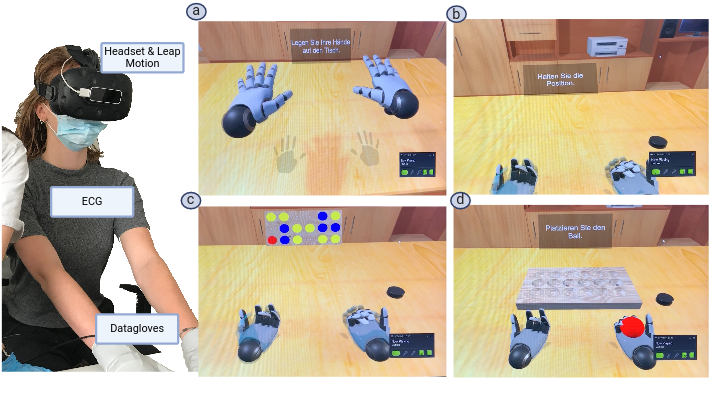
\includegraphics[width=15cm]{/home/perdices/Dokumente/Github/m-b_thesis/HU Thesis/figures/set_up_design.png}
    \put(-420,240){\textbf{I}} % Adjust (-20,340) to position "I" label as desired
    \put(-320,240){\textbf{II}} % Adjust (360,340) to position "II" label as desired
    \captionsetup{justification=justified, margin={2cm,2cm}, font={small}}
    \caption{IVR Memory-Motor Task: Panel I shows a participant wearing equipment. Panel II shows step (a) represents the acclimation period during initial setup and first-step calibration; (b) showcases the first-person perspective of the second calibration phase; (c) displays the 2D sketch for memorizing ball position; (d) presents the appearance of the ball and the 3D template for ball placement, marking the beginning of each trial.}
    \label{fig:looks}
\end{figure}
 
In a sequence of 105 trials, three conditions—congruent ($V=T$), incongruent ($V \neq T$), and visual-only ($V$)—were presented randomly and rapidly, each occurring 35 times. Each trial commenced upon positioning the ball in a hand, concluding only upon its precise placement on the designated template (refer to Figure \ref{fig:looks}). 

Given that an IVR task inherently involves proprioceptive signals, all conditions in the experiment integrate these signals and are thus multimodal. Consequently, the 'visual only' condition doesn't align with the unimodal classification commonly used in psychophysics literature. Nonetheless, for the sake of easier comparison to this literature in this thesis, I will refer to it as unimodal, and the congruent and incongruent conditions as bimodal.

\subsection*{Measures}
\subsubsection*{Immersive Virtual Reality (VR):}

Movement data from 3 devices was recorded (data gloves, Leap Motion device, and the HMD was collected). For movement analysis, only the wrist movements tracked by the Leap Motion device were considered, excluding the fingertips' magnetic tracking sensor data. All movements were recorded in an Euclidean coordinate system (X, Y, Z) with the original calibrating point set at (0, 0, 0). As each device had three coordinates, this provided a total of nine streaming sources of data (e.g., Headset X, Headset Y, Headset Z, and so on). Additionally, rotational data was recorded. Both sources are not included in the analysis since at the moment it does not help to compare with the race inequality model. 

Additionally, in the game output data, there are flags that signal if a button was pressed, if the ball is placed in the holder, and when the trial started. Trials where the error button was pressed were excluded from the analysis.

\subsubsection*{Questionnaires:}
Both of the described questionnaires are included in the appendix of this thesis for further reference. Questionnaire validation is outside the scope of this thesis:

\begin{enumerate}
\item[(i)] \textbf{Virtual Reality Subjective Evaluation Questionnaire:} This self-designed questionnaire comprises 26 items aimed at assessing the sense of reality experienced during the VR session. It explores factors like engagement level, hand movement, task difficulty, and other controlling aspects. Participants responded using a Likert scale rating them on a scale from 1 (Does Not Apply) to 7 (Totally Applies). The questions were organized in groups and inverted to confirm participants' responses. Both questionnaires can be found in the Appendix section.

\item[(ii)] \textbf{PRE/POST-Cybersickness Questionnaire:} This study employs a shortened version of the simulator sickness questionnaire \parencite{avpsy}. It utilizes a Likert scale ranging from one to four, featuring labels such as "not present," "somewhat," "clearly," and "very strongly." The questionnaire consists of 16 items, gauging symptoms like "fatigue" and "general discomfort," among others.
\end{enumerate}

\subsection*{Data Analysis}

\subsubsection*{Virtual Reality Subjective Evaluation}
The analysis of the questionnaire responses aimed to explore the impact of haptic gloves on reported immersion and related perceptions. Initially, raw questionnaire data were collected from 20 respondents, consisting of 27 questions rated on a scale from 1 to 7. Some participants did not answer all questions, thus creating specific missing values that were omitted. Statistical analysis included the calculation of descriptive statistics such as median ($\text{Mdn}$), mean ($\mu$), and standard deviation ($\sigma$) for each question. These statistics were instrumental in understanding the central tendencies and variability in respondents' perceptions. A full view of all answers can be found in the Supplements section.

\subsubsection*{Response Time}

All response times from the ball's entry into the scene until its disappearance were measured. Trials, where the error button was pressed, were excluded from the analysis. Before analysis, outliers were corrected by eliminating data points deviating more than 3 times the median absolute deviation (MAD), which is equivalent to 3 standard deviations assuming a normal distribution \parencite{Innes2019ACA}. Responses were not eliminated for being too fast; however, 13\% of trials were excluded due to excessive slowness. The final sample comprised 1826 response times (approximately 24 per condition per participant). After the removal of outliers, the response times for each condition were transformed into rates ($1/RT$).

The transformation method entails the inversion of the RT and aligns with prior studies \parencite{Innes2019ACA}. However, this transformation method is not exempt from criticism \parencite{Lo2015-fv}. This study prioritizes normality in error distribution over other factors such as property scale or interacting effects. This prioritization allowed for the direct application of repeated measures ANOVA within subjects. Yet, when the ANOVA results were ambiguous, a General Linear Mixed-Effect Model (GLMM) was additionally applied, as recommended by \textcite{Lo2015-fv}. By using GLMM, instead of imposing normality and eliminating error deviation, we allow the use of distributions that match the properties of the measured RT \parencite{Lo2015-fv}. I utilized the \textit{statsmodels} statistical package in Python, specifically the \textit{mixedlm} function, similar to other studies \parencite{RSE_FBI}. Although this analysis is not present in the reference study, the utilization of GLMM aims to provide clarity regarding the significance of the conditions and the study's power.

\subsubsection*{Redundancy Signal Effect and Race Model Inequality}

The Race Model statement is simple. It suggests that two different unimodal stimuli (e.g., vision, and touch) undergo processing in distinct sensory channels and race to trigger detection. If these two stimuli were presented simultaneously, then we would expect the fastest one to elicit the response (essentially, the one "winning the race"). Therefore, we would be right to expect inequalities (1) and (2) to be held:

\[
F_y(t) \leq F_x(t), \quad t > 0, \quad (1)
\]
\[
F_z(t) \leq F_x(t), \quad t > 0, \quad (2)
\]

A violation of the inequalities would require that two modalities presented at the same time have a faster response time than one of these modalities presented alone. This would indicate that the two modalities interacted in some way, thus explaining the faster response than a single modality on its own. Accurate knowledge of this is basic for understanding multisensory integration better.

Here, $F_x$ represents the cumulative density functions (CDFs) of reaction times (RT) in the individual stimulus conditions visual-only ($V$), respectively, while $F_y$ and $F_z$ denote the CDF of RT in the redundant-stimulus conditions congruent ($V=T$) and incongruent ($V \neq T$). According to race models, there's a possibility for $F_z(t)$ or $F_y(t)$ to closely approach $F_x(t)$ for small values of $t$, particularly in scenarios with strongly negative correlations in detection times \parencite{Ulrich2007}. However, even under these circumstances, the inequality must still hold as per the race models.

It is important to mention here that IVR does not allow the same experimental methodology as traditionally held in race model inequality studies. For example, a constant proprioceptive signal is inherent in the IVR design across all conditions, thus making absolute single modality impossible. Additionally, having only one single unimodal stimulus (vision) available prevents us from constructing the complete set of cases (single touch, single vision). Nevertheless, I make comparisons between the congruent and incongruent conditions with the single modality condition ($V$) based on the fact that they all have proprioceptive modality included, thus cancelling the effect out. Furthermore, constructing cumulative distribution functions allows for testing the statistical significance of these differences.

The process involved generating empirical cumulative density functions (CDFs) for three conditions—Bimodal pairs and Single Signal—and followed the steps outlined in literature \parencite{Ulrich2007}. The first steps were followed for every participant and every stimulus condition. Specifically, let $G_x$ be the individual CDF estimate of the visual-only condition, and $F_y$ and $F_z$ denote the redundant CDF for the incongruent and congruent conditions.

Consider a scenario where a set $\{x_1, x_2, \ldots , x_n\}$ of $n$ reaction times (RTs) has been recorded within condition $V$ for a specific participant. Arranging this sample in ascending order, from the smallest value to the largest—$x_1 \leq x_2 \leq \ldots \leq x_n$—one creates a step function. The second step involves using a step function to generate a cumulative frequency polygon. The final step is the estimation of percentiles and aggregation across participants. For a comprehensive breakdown and reference code, consult \cite{Ulrich2007}. Additionally, the code for this thesis is shared on GitHub.

To mimic the results from our reference paper \Cite{SALTAFOSSI2023108642}, I conducted a series of t-tests using individual participant data for the $F_x$, $F_y$, and $F_z$ values at each percentile level. Rather than examining areas under the curve, I focused on the raw values of $F_x$, $F_y$, and $F_z$. Furthermore, instead of emphasizing time bins, I opted to discuss percentile levels, given the differing time ranges compared to traditional RMI literature are longer because of answering times in IVR task.

\section*{Results}
\subsection*{Cibersickness Questionnaire}
 
We performed a paired-sample t-test to assess the cybersickness levels before (Pre) and after (Post) the Virtual Reality Experience. There was a significant difference in the scores between the Pre (M=1.10, SD=0.12) and Post (M=1.18, SD=0.19) conditions; $t(21)=-2.65$, $p = 0.015$. On average, the symptoms moved from "not present" to "somewhat present". 

\subsubsection*{Virtual Reality Subjective Evaluation Questionnaire}
Nineteen respondents answered 27 questions, rating them on a scale from 1 (Does Not Apply) to 7 (Totally Applies). The key facts from the Virtual Reality Subjective Evaluation Questionnaire are as follows:
    
The gloves seem to enrich the reported expirience as in question number 24 of the questionnaire, the reported score on the perceived immersion due to the haptic gloves was "Applies" ($\text{Mdn} = 6$, $\mu = 6$, $\sigma = 0.76$). Furthermore, question 19 over whether the task was considered enjoyable at least some of the time was also answered as "Applies" ($\text{Mdn} = 6$, $\mu = 5.4$, $\sigma = 1.04$).
        
Although then enriched expirience does not translate into percieved improved performance. Question 26 revealed that haptic feedback was perceived as either not significantly improving performance or having a "Neutral" effect ($\text{Mdn} = 3$, $\mu = 3.6$, $\sigma = 1.49$). Similarly, in question 12, the perception of haptic feedback improving response time was generally rated as "Neutral" ($\text{Mdn} = 3$, $\mu = 3.7$, $\sigma = 1.74$). In question 7, when asked about the impact on results, haptic feedback was perceived as "Not applicable" as well ($\text{Mdn} = 6$, $\mu = 6$, $\sigma = 0.76$).
    
Overall the memory task is percieved as not difficult. Notably, the assertion that it was very challenging to remember the position of the red ball ($\text{Mdn} = 2$, $\mu = 2.9$, $\sigma = 1.45$) was generally disagreed upon. Conversely, question 8, which asked the inverse question about the ease of remembering the location of the red ball ($\text{Mdn} = 5$, $\mu = 5.1$, $\sigma = 1.37$) aligns with its counterfactual and it is reported as highly easy. 
    
I suspect that questions about the easiness of the action are not clearly made. Relative to all other questions the highest variance was observed in question 13 ($\text{Mdn} = 5$, $\mu = 4.2$, $\sigma = 1.79$), indicating that haptic feedback made it easier to place the ball. Similarly, question 18, which inquired about the ease of counting heartbeats at the beginning of the experiment, also showed significant variance ($\text{Mdn} = 4$, $\mu = 4$, $\sigma = 1.79$). 
    
Overall, participants reported increased immersion and enjoyment as a result of the added gloves. However, there was no perceived enhancement in response attributed to the presence of the gloves and the IVR ball placing task was considered easy. Furthermore, the significant variation noted in participants' responses to the last two questions may suggest that some individuals are unsure about how easy it is to perform the specific task mentioned. For a more detailed breakdown, please refer to the supplementary section.
    
\subsection*{Influence of Touch Stimuli on Response Time}
\subsubsection*{General Performance}

Initially, I assessed the mistake rates in ball placement (balls placed in a different position than the one qued in the prompter) across different conditions to ensure their negligible impact on the experiment. The mistake rates were as follows: in the visual-only condition ($V$), it was $6.35\%$ ($\pm 0.99\%$, SEM); in the visual incongruent touch condition ($V \neq T$), it was $5.79\%$. Additionally, a one-way ANOVA indicated no significant effects ($ F \leq 0.08$, $p \geq 0.91$) between all three experimental conditions (congruent, incongruent and visual-only). This task is considerably more complex than a simple yes-no detection task. Therefore, to some extent, we anticipate a higher mistake rate. Nevertheless, these rates remain notably low and were not subjected to further analysis.

To investigate whether the experimental manipulations successfully affected the RT, I conducted a one-way repeated-measures ANOVA. The test revealed a significant main effect for the stimulus ($F(2,38) = 3.4$, $p \leq 0.043$, $\eta p^2 = 0.15$). The median response time for the 'Congruent' condition ($V=T$) was the fastest ($3236$ ms $\pm 456$ ms), followed by the 'Incongruent' ($V \neq T$) condition ($3268$ ms $\pm 470$), while the slowest was observed in the absence of haptic stimuli 'None' ($V$) ($3284$ ms $\pm 463$). Thus, the experimental conditions significantly influenced response times, as illustrated in Figure \ref{fig:error}. However, post hoc Tukey HSD tests did not reveal any specific pairwise differences. While an overall difference among conditions was observed, specific pairwise differences were not identified.

\begin{figure}[!ht]
    \centering
    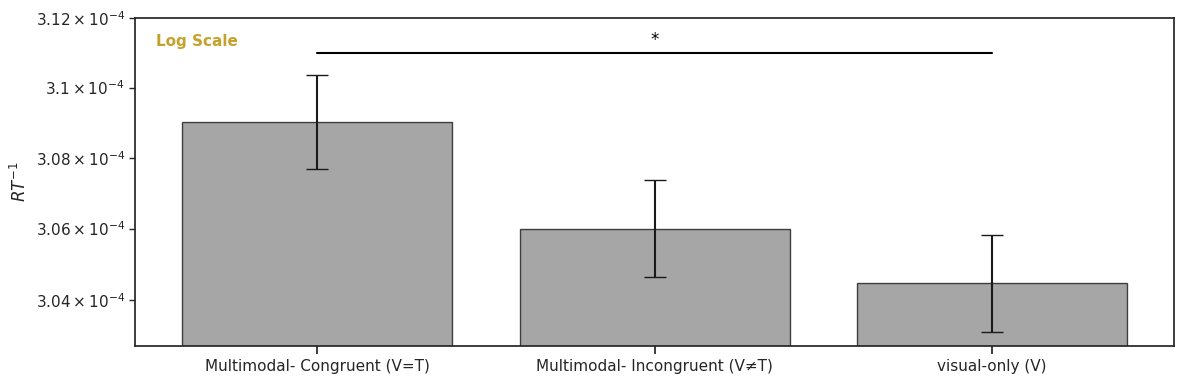
\includegraphics[width=15cm]{/home/perdices/Dokumente/Github/m-b_thesis/HU Thesis/figures/bar_erros_bars_stimulus_constructions.png}
    \captionsetup{justification=justified, margin={2cm,2cm}, font={small}}
    \caption{One-way repeated-measures ANOVA using $RT^{-1}$. The test revealed a significant main effect for the conditions ($F(2,38) = 3.4$, $p \leq 0.043$, $\eta p^2 = 0.15$)}
    \label{fig:error}
\end{figure}

Given the absence of identified specific pairwise differences in the post hoc analysis, I conducted a more comprehensive investigation using a Generalized Linear Mixed Model (GLMM).
The linear mixed model analysis aimed to assess the impact of conditions (($V=T$), ($V \neq T$), ($V$)) on response times. The model included condition as a fixed effect and participant as a random effect, with the 'Congruent' condition serving as the reference category.

Although this specific analysis method was not employed in the referenced paper \parencite{SALTAFOSSI2023108642}, it offers numerous advantages for multilevel research designs. It addresses, for example, the issue of the linear relationship between the standard deviation of RT and mean RT, characterized by an increasing spread in residuals for longer predicted RT \parencite{Lo2015-fv}.

The model coefficient for the 'None' ($V$) condition ($\beta = 45.726, SE = 22.594, p = 0.043$) reached statistical significance at the conventional level ($\alpha =0.05 $) when compared to the 'Congruent' ($V=T$) condition. This suggests a significant difference in response times between the 'None' and 'Congruent' conditions. The coefficient for the 'Incongruent' condition ($\beta = 32.975, SE = 22.686, p = 0.146$) did not reach conventional levels of significance. 

Thus, the 'Congruent' condition demonstrated significantly faster performance compared to the visual-only condition. This outcome aligns with the expected results according to the RSE. However, the findings present a mixed perspective. Despite this significant contrast, the more stringent post hoc Tukey HSD tests revealed no notable differences between pairwise conditions. Additionally, the GLMM indicated significance solely between the 'Congruent' ($V=T$) and visual-only ($V$) conditions and not between the 'Congruent' ($V=T$) and 'Incongruent' ($V \neq T$) conditions. We should consider that median time differences between conditions range between 30 to 50 milliseconds. Now that we have validated the condition. To gain a deeper understanding of the results and nest them in the literature the next section of RMI and CDF analysis will aim to achieve this. 

\subsubsection*{Race Model Inequeality}

In this section, I utilize the Cumulative Distribution Function (CDF) from the Race Model Inequality (RMI) model to evaluate the significance of differences between conditions at different time points ($t$). The t-test conducted between the three experimental conditions revealed significant differences between the 'Congruent' and visual-only ($V=T$ ; $V$) conditions, but no significant differences emerged between the 'Congruent' and 'Incongruent' conditions ($V=T$ ; $V \neq T$). The results between $F_x$ and $F_z$ ($V$ ; $V=T$) are presented in Table \ref{tab:response-time-range}, which illustrates the results for all time frames and percentiles. Notably, significant differences emerged between $F_x$ and $F_y$ from the 16th percentile onwards. Interestingly, for this percentile (as depicted in Figure \ref{fig:CDF}), the single modality visual ($V$) appears to be faster than the bimodal incongruent condition ($V \neq T$), suggesting a potential violation of the RMI principle. Conversely, from the 40th percentile onwards, both redundant signals consistently demonstrate faster response times compared to the unimodal signal, aligning with our expectations based on the RSE. It's important to note that when considering the distribution of all response times, the highest density is observed between 3100 and 3200 ms, accounting for 33\% of all response times.

\begin{table}[!ht]
    \centering
    \adjustbox{max width=\textwidth}{
    \begin{tabular}{ccccccccc}
    \hline
    \textbf{Percentile Estimation} & \textbf{$F_z$ Time Range (ms)} & \textbf{$F_z$ Min Max Diff (ms)} & \textbf{$F_z$ T-value} & \textbf{$F_z$ p-value} & \textbf{$F_y$ Time Range (ms)} & \textbf{$F_y$ Min Max Diff (ms)} & \textbf{$F_y$ T-value} & \textbf{$F_y$ p-value}  \\ \hline
    10 & (3070, 3621) & 551 & 1.19 & 0.12 & (3121, 3907) & 786 & 1.1 & 0.14 \\
    13 & (3078, 3626) & 548 & 1.31 & 0.1 & (3123, 3969) & 846 & 0.79 & 0.22 \\
    16 & (3084, 3648) & 564 & 1.88 & 0.04* & (3130, 4171) & 1041 & 0.92 & 0.18 \\
    19 & (3086, 3687) & 600 & 2.04 & 0.03* & (3141, 4352) & 1211 & 0.96 & 0.18 \\
    20 & (3087, 3708) & 621 & 2.01 & 0.03* & (3153, 4645) & 1492 & 0.96 & 0.17 \\
    23 & (3092, 3748) & 656 & 1.97 & 0.03* & (3176, 4948) & 1772 & 0.99 & 0.17 \\
    26 & (3094, 3760) & 665 & 2.06 & 0.03* & (3202, 5060) & 1857 & 1.04 & 0.16 \\
    29 & (3098, 3766) & 668 & 2.03 & 0.03* & (3221, 5184) & 1963 & 1.33 & 0.1 \\
    30 & (3099, 3768) & 668 & 2.02 & 0.03* & (3241, 5290) & 2049 & 1.34 & 0.1 \\
    33 & (3104, 3814) & 709 & 2.11 & 0.02* & (3264, 5391) & 2127 & 1.02 & 0.16 \\
    36 & (3106, 3838) & 732 & 2.08 & 0.03* & (3287, 5558) & 2271 & 0.95 & 0.18 \\
    39 & (3111, 3846) & 735 & 1.83 & 0.04* & (3311, 5739) & 2427 & 1.13 & 0.14 \\
    40 & (3114, 3848) & 734 & 1.79 & 0.04* & (3336, 5884) & 2548 & 1.19 & 0.12 \\
    43 & (3119, 3861) & 741 & 1.74 & 0.05* & (3361, 6067) & 2706 & 1.16 & 0.13 \\
    46 & (3121, 3907) & 786 & 1.55 & 0.07 & (3396, 6271) & 2946 & 0.85 & 0.2 \\
    49 & (3123, 3969) & 846 & 1.36 & 0.09 & (3431, 6503) & 3181 & 0.48 & 0.32 \\
    50 & (3124, 3978) & 855 & 1.33 & 0.1 & (3466, 6723) & 3421 & 0.29 & 0.39 \\
    60 & (3130, 4171) & 1041 & 1.25 & 0.11 & (3499, 6989) & 3680 & 0.91 & 0.19 \\
    70 & (3141, 4352) & 1211 & 1.21 & 0.12 & (3530, 7310) & 3939 & 0.4 & 0.35 \\
    80 & (3153, 4645) & 1492 & 1.47 & 0.08 & (3560, 7674) & 4253 & -0.54 & 0.7 \\
    90 & (3176, 4948) & 1772 & 0.53 & 0.3 & (3589, 8081) & 4632 & -0.27 & 0.61 \\ \hline
    \end{tabular}}
    \captionsetup{justification=justified, margin={2cm,2cm}, font={small}}
    \caption{Let $G_x$ be the individual CDF estimate of the visual-only condition, and $F_y$ and $F_z$ denote the redundant CDF for the incongruent and congruent conditions. Each row represents a percentile. Each t-test evaluates a significant difference compared to $G_x$, * indicates significant p-values.Estimations are for $F_y$ and $F_z$}
    \label{tab:response-time-range}
\end{table}


\begin{figure}[!ht]
    \centering
    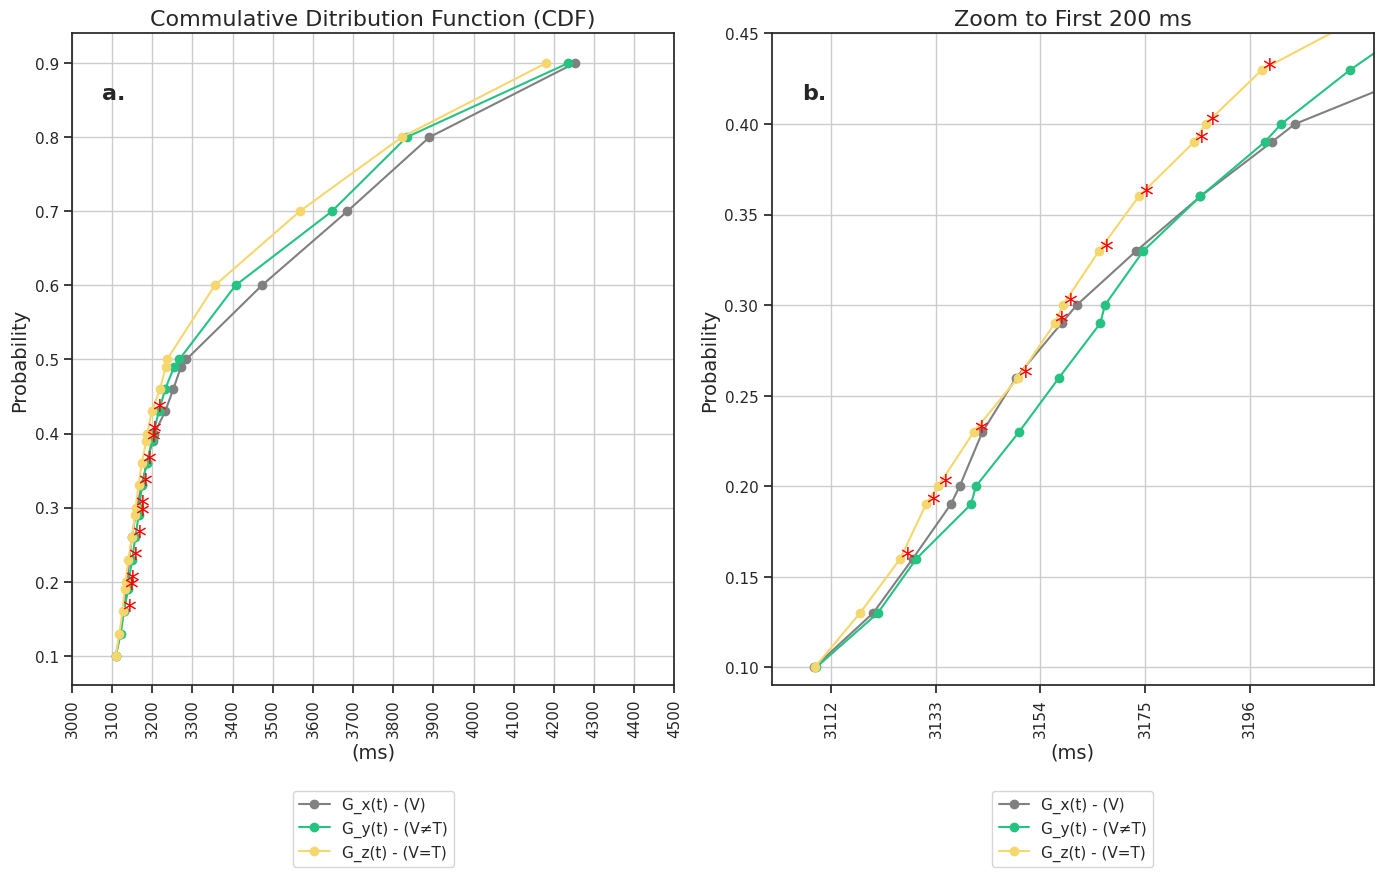
\includegraphics[width=\textwidth]{/home/perdices/Dokumente/Github/m-b_thesis/HU Thesis/figures/CDF.png}
    \captionsetup{justification=justified, margin={2cm,2cm}, font={small}}
    \caption{ (a.) Displays the estimated percentile points for each of the three functions of interest: $G_x$, $F_y$, $F_z$, considering all participants. (b.) Is a zoom in the first 100 ms of the entire RT range. Acording to the RSE, the CDF $G_x$ of the visual-only ($V$) condition should be under $F_y$, $F_z$ at all moments. Our data shows that is not the case for the first 100 ms of the entire RT range.}
    \label{fig:CDF}
\end{figure}


\section*{Discussion}

I have carefully analyzed the validity of a haptic glove as a stimuli in an IVR memory task and compared the results to previous research on multisensory integration in the context of RSE and RMI models. The goal of this research is to bridge the gap between cognitive and psychophysical studies and improve the use of IVR as a tool for developing more advanced cognitive psychophysics.

To accomplish this goal, the task required participants to remember a location and immediately place an appearing red ball over this location in a 3D template. As mentioned in the task section, the condition is designed so that a passive vibrotactile stimulus is activated when a red ball visually appears in the hand. The conditions are built as follows: There is a match between the visual location of the ball and the vibration of the glove, then it's called congruent visual-tactile stimuli ($V=T$). When there is a mismatch between the location of the ball and the vibration of the glove, then it's called incongruent visual-tactile stimuli ($V \neq T$). Finally, when there is no vibration in any glove but only IVR visual cues, then the condition is called visual-only stimuli ($V$). The study employs a within-subject experimental design with the three aforementioned conditions. Additionally, the participants answered a cybersickness questionnaire.

Over a third of the trials were answered within 3100 ms and 3200 ms. To validate stimulus construction, I analyzed and modeled the reaction times for unimodal and bimodal stimuli. The results showed a significant difference between the conditions, but no significant distinctions were found when attempting to identify pairwise differences using a Tukey HSD test. However, a GLMM indicated a notable difference between the visual-only ($V$) and visual-touch congruent ($V=T$) conditions. No significant variances observed between the incongruent ($V \neq T$) and visual-only ($V$) conditions.

To compare the IVR set-up with existing literature I followed the steps outlined in my reference study \parencite{SALTAFOSSI2023108642}. Using the RSE and RMI models, we can use the cumulative distribution function (CDF) to compare the probability that a response time is equal or less at period time $t$. By doing so for our three conditions, we can validate the set-up against existing psychophysical literature.

The RMI analysis indicates a significant disparity in the cumulative distribution functions (CDF) between conditions when conducting a between-participants t-test for $F_x$ and $F_z$. This discrepancy occurs specifically within the timeframe of 3100 ms to 3200 ms, rather than before or after. Moreover, no significant differences were observed for $F_x$ and $F_y$ during this 100 ms period or thereafter.

Descriptively, the relationship between the visual-only ($V$) and congruent condition ($V=T$) remains consistent across the entire range of reaction times (RT), aligning with the Race Model inequality (RMI). However, this pattern doesn’t hold for the RT relation between the incongruent condition ($V \neq T$) and the visual-only condition ($V$), where within the first 100 ms of the complete RT range, the single visual condition displays faster responses than the bi-modal incongruent condition ($V \neq T$), potentially breaching the expected inequality. In later response times, the incongruent condition is faster than the unimodal visual-only condition, as anticipated. This again raises the question of a possible violation of the RMI model. Particularly as a bimodal condition ($V \neq T$) demonstrates slower responses compared to an unimodal condition ($V$).

I have identified evidence suggesting that the incongruent condition contradicts the predictions of the RMI model within the initial 100 milliseconds of the reaction time (RT) range. However, given the significance lies at the boundary and the effects are relatively minor, I am inclined to seek additional validation to strengthen this interpretation. Another study by \cite{RSE_FBI} investigating embodiment illusion (the reported feeling of seeing one body where is not) yielded similar results concerning the irrelevance of stimuli for reaction times (RT). Their hypothesis suggests that the absence of a difference in the Race Model Inequality (RMI) between congruent and incongruent conditions could be due to the mere simultaneous occurrence of visual and vibrotactile stimuli. This simultaneous presence might suffice for multisensory integration, regardless of whether these multisensory stimuli are functionally linked at a higher level or not (e.g., touch in the hand holding the ball) \parencite{RSE_FBI}. This explanation seems to apply to the responses after the 40th percentile and the overall results, but it doesn't account for the observed first 40th percentile of answers, indicating a potential violation of the RMI.

Some of this study's limitations come from the integration of different devices. The latencies between them are not the same, thus possibly creating data loss or duplicate repeated values for every $t$ in time. This could affect the results in the analysis, especially for psychophysical experimental design. Other considerations need to be held as experiments using IVR will include proprioceptive cues which must be considered when establishing parallels between current and past studies. Finally, each trial in our IVR study spans a longer time frame compared to traditional psychophysics experiments (with a mean duration of 3400 ms versus the typical 200 ms). This extended duration contributes to increased variance and skewness in reaction times (RT) which needs to be addressed as I did in this thesis. Nonetheless, this makes it harder to compare to other psychophysics experiments.

A new design should pay attention to the latencies between all interfaces (e.g., ECG, Gloves, HMD) and integrate them accordingly, considering that the mean differences between somatosensory conditions might be as small as 20 ms. Thus latency integration issues over 7 ms might hinder the results. The experimental design should also measure RT between the trial start and the initiation of movement so the mean RT and variance shorten, thus avoiding the skewness problem and increasing the significance of the results. Additionally, increasing the sample of future research, involving, for instance, 60 participants to be able to come to more definite conclusions regarding the central hypotheses investigated here (RSE, RMI). A further interesting question to investigate is whether the heart cycle has an effect on RMI violations during multisensory integration.

\newpage
\begin{figure}[ht]
        \centering
        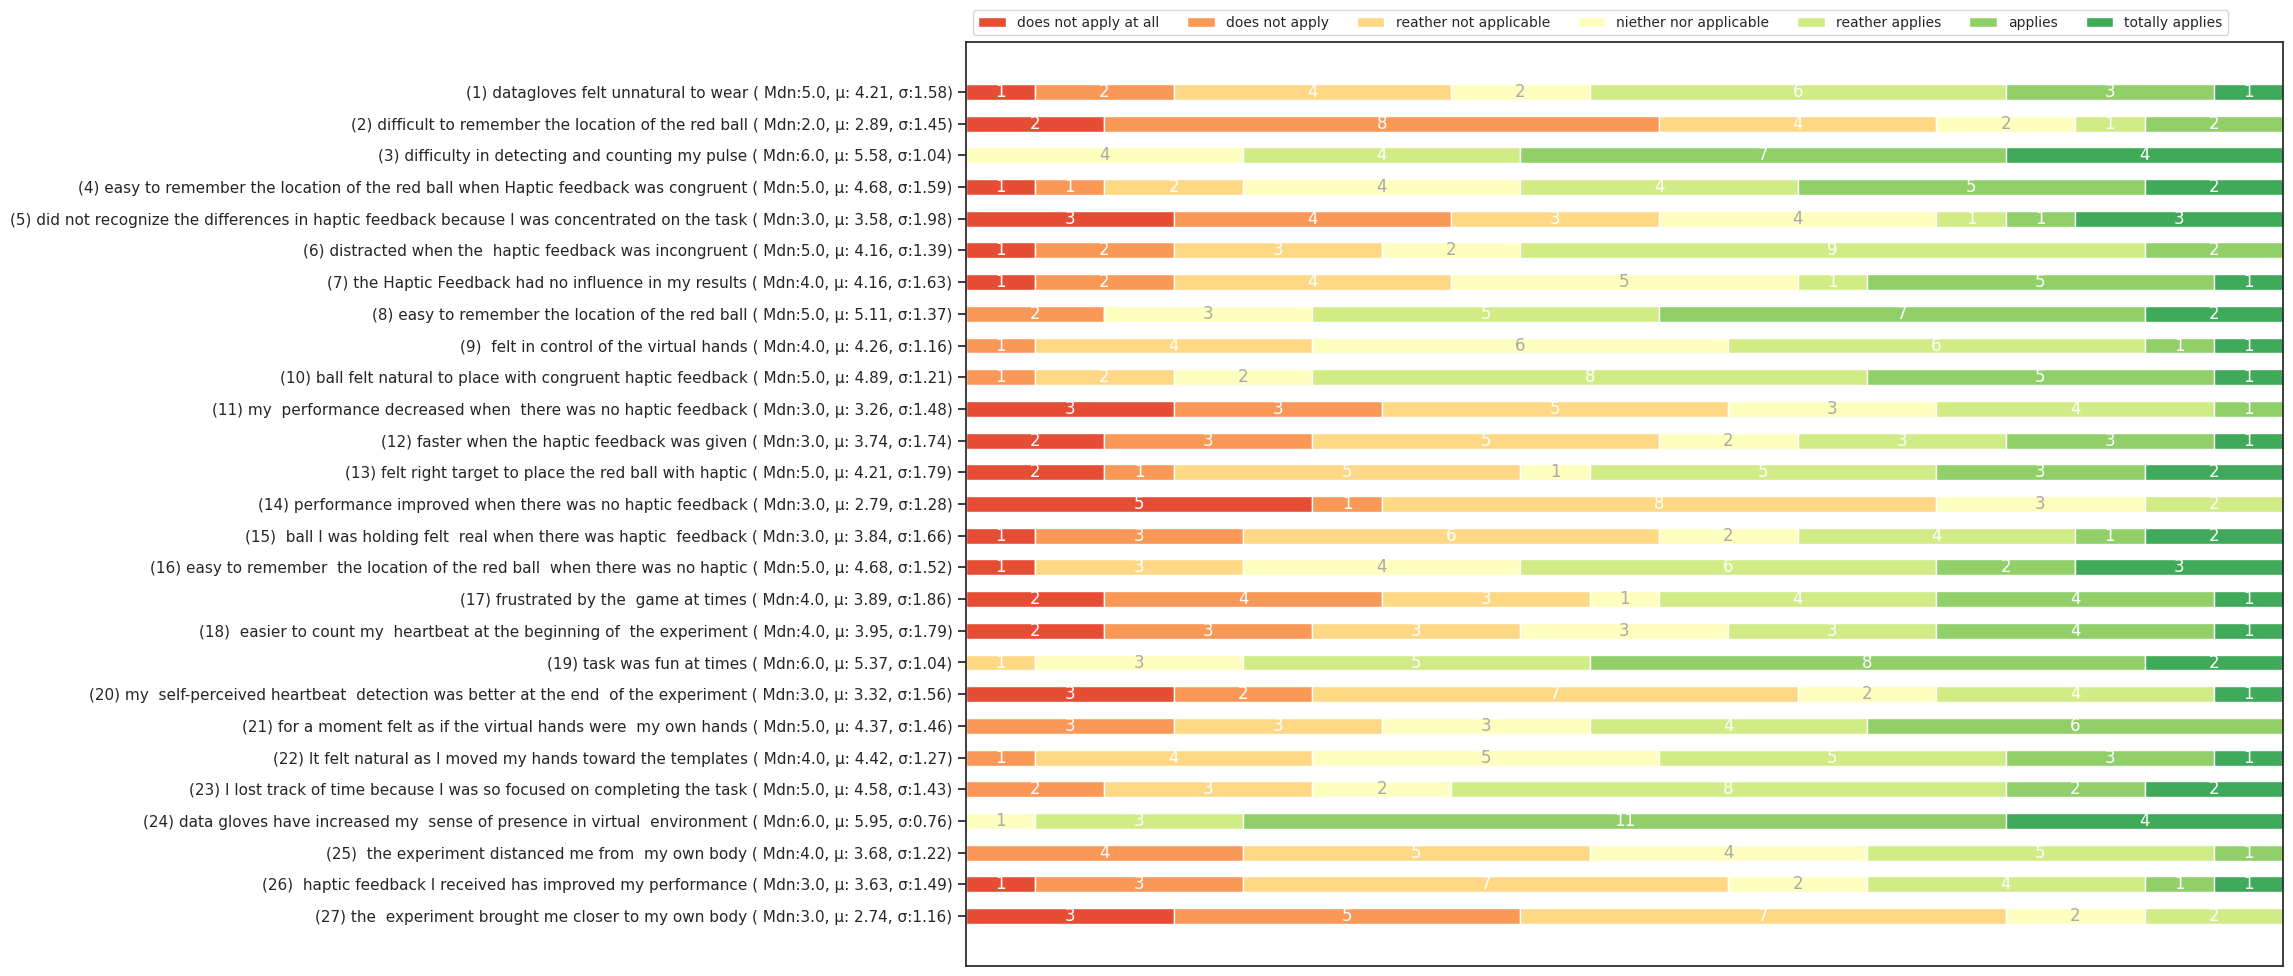
\includegraphics[angle=90, width=\textwidth, height=20cm, keepaspectratio]{/home/perdices/Dokumente/Github/m-b_thesis/HU Thesis/figures/questionaire_fig.png}
        \captionsetup{justification=justified, margin={2cm,2cm}, font={small}}
        \caption{Results: Virtual Reality Subjective Evaluation Questionnaire}
        \label{fig:quest}
\end{figure}
\pagebreak


%-------- CREATING BIBLIOGRAPHY

\paragraph{\textbf{References}}
\printbibliography[heading=none]

%-------- CREATING Apendix

\pagebreak
\vspace*{\fill}
\section*{\centering Additional Material}
\vspace*{\fill}



\end{document}

